\subsection{Summary} \label{section:license-abstraction}
All license verification libraries are working inside the application and query a trusted source.
For the \gls{lvl} and \textit{Zirconia}, the trusted source is a server while for \textit{Kiwi} it is the store application.
They do not prevent redistribution or copying, but enforce the authorization when the application is run.
The result of the verification is always binary, from the view of successfully run the application, it is even unary.
Only one result is acceptable, which is license verified.
In the further analysis it will be shown that this unary mechanism is an easy target for attacks, such as executed by \gls{luckypatcherg}.
\newline
The functionality of the libraries and in fact any test can be abstracted as a simple \textit{yes/no} check as seen in figure~\ref{fig:verificationNow}.
\begin{figure}[h]
    \centering
    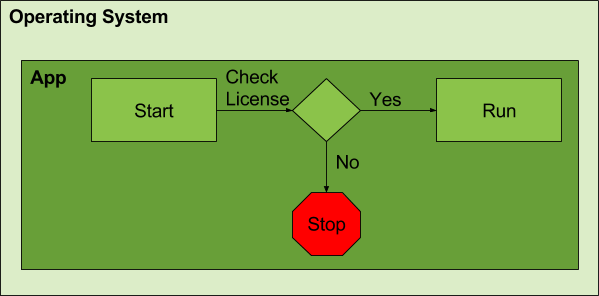
\includegraphics[width=0.8\textwidth]{data/verificationNow.png}
    \caption{Abstraction of the current license verification mechanism. The library is represented by \textit{(1)}.}
    \label{fig:verificationNow}
\end{figure}
